% Editable source for local_law.pdf, written by make_local_figure.py from inputs/local_decisive_test.json
\documentclass[tikz,border=6pt]{standalone}
\usepackage[T1]{fontenc}
\begin{document}
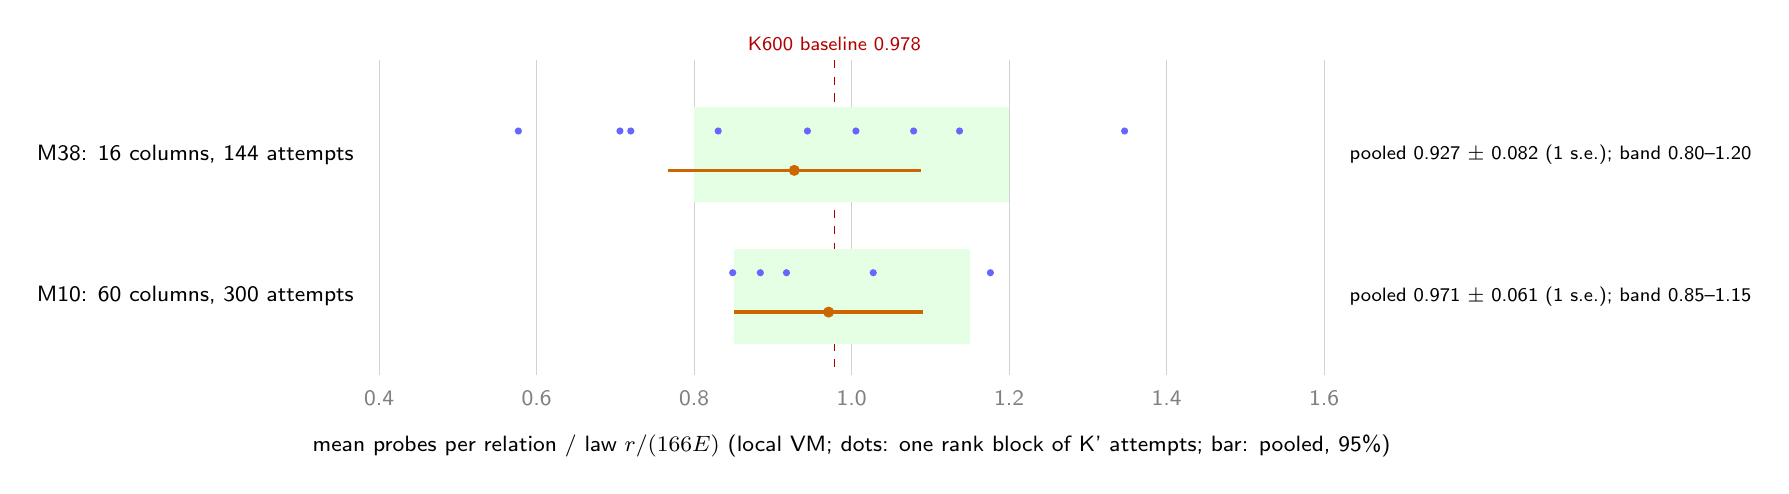
\begin{tikzpicture}[font=\sffamily\footnotesize,x=1cm,y=-1cm]
\draw[gray!35] (0.000,-0.4) -- (0.000,3.6); \node[gray] at (0.000,3.9) {0.4};
\draw[gray!35] (2.000,-0.4) -- (2.000,3.6); \node[gray] at (2.000,3.9) {0.6};
\draw[gray!35] (4.000,-0.4) -- (4.000,3.6); \node[gray] at (4.000,3.9) {0.8};
\draw[gray!35] (6.000,-0.4) -- (6.000,3.6); \node[gray] at (6.000,3.9) {1.0};
\draw[gray!35] (8.000,-0.4) -- (8.000,3.6); \node[gray] at (8.000,3.9) {1.2};
\draw[gray!35] (10.000,-0.4) -- (10.000,3.6); \node[gray] at (10.000,3.9) {1.4};
\draw[gray!35] (12.000,-0.4) -- (12.000,3.6); \node[gray] at (12.000,3.9) {1.6};
\draw[red!70!black,dashed] (5.780,-0.4) -- (5.780,3.6);
\node[red!70!black,font=\sffamily\scriptsize,anchor=south] at (5.780,-0.4) {K600 baseline 0.978};
\node at (6,4.5) {mean probes per relation / law $r/(166E)$ (local VM; dots: one rank block of K' attempts; bar: pooled, 95\%)};
\fill[green!10] (4.000,0.20) rectangle (8.000,1.40);
\node[anchor=east] at (-0.2,0.80) {M38: 16 columns, 144 attempts};
\fill[blue!60] (3.195,0.50) circle (1.3pt);
\fill[blue!60] (9.466,0.50) circle (1.3pt);
\fill[blue!60] (7.370,0.50) circle (1.3pt);
\fill[blue!60] (4.305,0.50) circle (1.3pt);
\fill[blue!60] (3.057,0.50) circle (1.3pt);
\fill[blue!60] (6.054,0.50) circle (1.3pt);
\fill[blue!60] (5.438,0.50) circle (1.3pt);
\fill[blue!60] (1.767,0.50) circle (1.3pt);
\fill[blue!60] (6.787,0.50) circle (1.3pt);
\draw[very thick,orange!80!black] (3.665,1.00) -- (6.877,1.00);
\fill[orange!80!black] (5.271,1.00) circle (2pt);
\node[anchor=west,font=\sffamily\scriptsize] at (12.2,0.80) {pooled 0.927 $\pm$ 0.082 (1 s.e.); band 0.80--1.20};
\fill[green!10] (4.500,2.00) rectangle (7.500,3.20);
\node[anchor=east] at (-0.2,2.60) {M10: 60 columns, 300 attempts};
\fill[blue!60] (5.172,2.30) circle (1.3pt);
\fill[blue!60] (6.274,2.30) circle (1.3pt);
\fill[blue!60] (7.762,2.30) circle (1.3pt);
\fill[blue!60] (4.840,2.30) circle (1.3pt);
\fill[blue!60] (4.489,2.30) circle (1.3pt);
\draw[very thick,orange!80!black] (4.508,2.80) -- (6.907,2.80);
\fill[orange!80!black] (5.707,2.80) circle (2pt);
\node[anchor=west,font=\sffamily\scriptsize] at (12.2,2.60) {pooled 0.971 $\pm$ 0.061 (1 s.e.); band 0.85--1.15};
\end{tikzpicture}
\end{document}
